\documentclass[12pt,a4paper]{article}
\PassOptionsToPackage{hyphens}{url}

\usepackage[utf8]{inputenc}
\usepackage[T1]{fontenc}
\usepackage{lmodern}
\usepackage[margin=2.5cm]{geometry}
\usepackage{amsmath,amssymb,amsthm,mathtools,bm}
\usepackage{booktabs,graphicx,caption,multirow}
\usepackage{microtype}
\usepackage{setspace}
\usepackage[authoryear,round]{natbib}
\usepackage[hidelinks]{hyperref}
\usepackage{url}
% Auto-generated by scripts/run_all.py -- do not edit by hand
\newcommand{\annualRevUSD}{2.76}
\newcommand{\betaCorrHi}{0.54}
\newcommand{\betaDKHi}{0.40}
\newcommand{\betaDKLo}{0.47}
\newcommand{\betaInternet}{0.51}
\newcommand{\betaKappaOne}{0.38}
\newcommand{\betaMax}{0.77}
\newcommand{\betaMin}{0.35}
\newcommand{\betaRevenue}{0.57}
\newcommand{\betaSigmaHi}{0.35}
\newcommand{\betaSigmaLo}{0.57}
\newcommand{\betaStar}{0.44}
\newcommand{\betaStarRev}{0.77}
\newcommand{\betaStarTigo}{0.48}
\newcommand{\claroShare}{48.7}
\newcommand{\claroThreshold}{41.0}
\newcommand{\coltelLossPct}{19}
\newcommand{\coltelLossUSD}{69}
\newcommand{\coltelS}{415}
\newcommand{\csGainPrefVsStd}{589}
\newcommand{\csMy}{746}
\newcommand{\csPref}{753}
\newcommand{\csSA}{858}
\newcommand{\csStd}{165}
\newcommand{\dCS}{907}
\newcommand{\dHHI}{200}
\newcommand{\dWMy}{374}
\newcommand{\dWPref}{359}
\newcommand{\dWSA}{331}
\newcommand{\gammaFactor}{8.51}
\newcommand{\gapSAKappaOne}{12}
\newcommand{\hhiMobile}{3,314}
\newcommand{\hhiPref}{3,148}
\newcommand{\hhiSA}{3,124}
\newcommand{\hhiStd}{3,277}
\newcommand{\impliedElasticity}{1.39}
\newcommand{\kappaBase}{0.77}
\newcommand{\lamZeroBeta}{0.77}
\newcommand{\mD}{818}
\newcommand{\mDoverE}{1.46}
\newcommand{\mE}{561}
\newcommand{\nEval}{10,000}
\newcommand{\netDropPref}{93}
\newcommand{\netLossPrefPct}{46}
\newcommand{\netMy}{129}
\newcommand{\netPref}{109}
\newcommand{\netPrefCorrHi}{150}
\newcommand{\netSA}{0}
\newcommand{\netStd}{202}
\newcommand{\pDPref}{17}
\newcommand{\pDStd}{82}
\newcommand{\pEPref}{83}
\newcommand{\pESA}{95}
\newcommand{\pEStd}{18}
\newcommand{\pEStdCorrHi}{3}
\newcommand{\pNoSA}{5}
\newcommand{\pairCvsE}{818}
\newcommand{\pairMvsC}{561}
\newcommand{\pairMvsT}{774}
\newcommand{\pairTvsC}{611}
\newcommand{\pairTvsM}{774}
\newcommand{\rZero}{333}
\newcommand{\regular}{yes}
\newcommand{\reserveBetaMax}{0.47}
\newcommand{\reserveBetaMin}{0.44}
\newcommand{\reserveWMax}{362}
\newcommand{\reserveWMin}{306}
\newcommand{\revGainAbs}{45}
\newcommand{\revGainPct}{22}
\newcommand{\scaleFactor}{17,695}
\newcommand{\shareMyerson}{96}
\newcommand{\sigmaMax}{0.6}
\newcommand{\sigmaMin}{0.1}
\newcommand{\wGainCorrHi}{480}

\newcommand{\repourl}{\url{https://github.com/hhernandezl-eco/Auctions-and-Privatization}}

\newtheorem{proposition}{Proposition}
\newtheorem{lemma}{Lemma}
\theoremstyle{definition}
\newtheorem{assumption}{Assumption}
\theoremstyle{remark}
\newtheorem{remark}{Remark}

\newcommand{\E}{\mathbb{E}}
\renewcommand{\Pr}{\mathbb{P}}
\newcommand{\us}{US\$}
\captionsetup{font=small,labelfont=bf}
\setcounter{secnumdepth}{2}

\title{Privatising under dominance: bid preferences in telecommunications auctions with downstream competition}
\author{Hernando Hern\'andez Lasso\\[2pt]
\small Facultad de Ciencias Econ\'omicas, Universidad Nacional de Colombia, Bogot\'a, Colombia\\
\small \texttt{hernandezlassohernando@gmail.com}}
\date{}

\begin{document}
\maketitle

\begin{abstract}
\noindent When a government sells a telecommunications asset to bidders that compete downstream, an incumbent's willingness to pay includes the value of denying the asset to its rivals. We embed a dominant-strategy ascending auction in a capacity-constrained Cournot market and show that the dominant firm's valuation is pure preemption, exceeds that of a challenger, and leads to an allocation that raises concentration and lowers consumer surplus. We derive the welfare-weighted Myerson mechanism for general valuation distributions, prove that a multiplicative bid preference is incentive compatible and discriminates in the optimal direction, and obtain closed forms for the uniform case, in which a preference recovers exactly three quarters of the optimal revenue gain. Calibrated to official data for the Colombian mobile market (Claro: \claroShare\% of lines; HHI \hhiMobile), a Monte Carlo study of \nEval{} auctions shows that, with a cost of public funds of 0.3, the optimal preference ($\beta^*=\betaStar$) lowers the incumbent's winning probability from \pDStd\% to \pDPref\%, costs the State \us\netDropPref{} million in expected proceeds, raises consumer surplus by \us\csGainPrefVsStd{} million, and attains \shareMyerson\% of the Myerson welfare gain; barring the incumbent is dominated. A revenue-maximising State would still favour the challenger, with a milder preference ($\beta^*=\betaStarRev$).
\end{abstract}

\medskip
\noindent\textbf{Keywords:} auctions; privatisation; bid preferences; market dominance; telecommunications; Colombia\\
\textbf{JEL classification:} D44, L96, L33, L51, H82

\onehalfspacing

%% ---------------------------------------------------------------------------
\section{Introduction}\label{sec:intro}

Selling a state-owned telecommunications operator, or the spectrum and network it holds, is a one-shot allocation problem with long-lived consequences for market structure. The bidders are almost never strangers to each other: they are the operators that will compete in the same retail market after the sale. An incumbent with a dominant position may therefore value the asset not because it can use it better, but because winning it keeps the asset away from the firm that would otherwise discipline its prices. A seller that ignores this motive and simply awards the asset to the highest bidder risks reproducing, and entrenching, the concentration it hoped to reduce.\footnote{This paper builds upon and substantially revises an earlier working paper in Spanish \citep{hernandez2021}, correcting its empirical calibration and analytical derivations.}

This paper studies how a government that privatises a telecommunications asset should design the auction when one bidder is dominant ex ante. We make three contributions. First, we \emph{endogenise} the asymmetry between bidders. Instead of assuming that a strong bidder draws valuations from a distribution with a higher support, we derive bidders' willingness to pay from a downstream capacity-constrained Cournot game in which market dominance is the incumbent's capacity slack (Section~\ref{sec:model}). In this model, the incumbent's willingness to pay is \emph{pure preemption}: extra capacity is useless to it, but denying that capacity to a constrained challenger preserves the incumbent's margin (Proposition~\ref{prop:preemption}, in the spirit of \citealt{gilbertnewbery1982}). The same preemption makes the allocation by willingness to pay inefficient: the incumbent outbids the challenger exactly when the challenger's capacity expansion would raise output and consumer surplus the most.

Second, we characterise the seller's optimal response. The welfare-weighted Myerson mechanism for general, possibly asymmetric, valuation distributions \citep{myerson1981,bulowroberts1989} awards the asset to the bidder with the highest virtual value plus a consumer-surplus premium (Proposition~\ref{prop:myerson}). A multiplicative bid preference---a policy that governments already use---is dominant-strategy incentive compatible and discriminates in the optimal direction whenever the incumbent is stronger in the hazard-rate sense and consumer surplus is valued (Proposition~\ref{prop:handicap}). For uniform valuations we obtain closed forms: a preference recovers exactly three quarters of the gain from optimal discrimination for every degree of asymmetry (Proposition~\ref{prop:uniform}).

Third, we quantify the policy trade-off for Colombia. We calibrate the downstream stage to the official quarterly bulletin of the Ministry of ICT (MinTIC) for the fourth quarter of 2020 and simulate \nEval{} auctions for each of three counterfactual regimes: a standard ascending auction, an auction with an optimally chosen bid preference for the challenger, and a set-aside that bars the dominant operator (Section~\ref{sec:results}). With a cost of public funds of 0.3, the preference cuts the incumbent's chance of winning from \pDStd\% to \pDPref\%, costs the State \us\netDropPref{} million in expected proceeds, and raises discounted consumer surplus by \us\csGainPrefVsStd{} million. It attains \shareMyerson\% of the welfare gain of the Myerson benchmark and dominates barring the incumbent.

The paper is organised as follows. Section~\ref{sec:lit} reviews the literature, Section~\ref{sec:background} summarises the institutional facts we use, Sections~\ref{sec:model} and~\ref{sec:theory} present the model and results, Sections~\ref{sec:calibration} and~\ref{sec:results} the calibration and counterfactuals, and Section~\ref{sec:discussion} discusses policy implications and two extensions: more than one challenger and an informational advantage \citep{emw1983}.

%% ---------------------------------------------------------------------------
\section{Related literature}\label{sec:lit}

\paragraph{Optimal and asymmetric auctions} \citet{myerson1981} and \citet{rileysamuelson1981} characterise revenue-maximising auctions with asymmetric independent private values; the optimal mechanism favours the weaker bidder whenever the stronger one is stronger in the hazard-rate sense \citep{bulowroberts1989,maskinriley2000}. \citet{cantillon2008} shows how asymmetry affects revenue in standard formats, and equilibrium existence and uniqueness for asymmetric first-price auctions are in \citet{lebrun1999} and \citet{maskinriley2003}, with analytical and numerical solutions in \citet{kaplanzamir2012} and \citet{marshall1994}. \citet{bulowklemperer1996} show that adding a bidder is worth more than any reserve price, a force that motivates entry-friendly designs such as ours. We differ in deriving the asymmetry from the downstream market rather than positing it, and in adding a consumer-surplus term to the seller's objective.

\paragraph{Externalities and downstream interaction} \citet{jehielmoldovanu2000} analyse auctions in which buyers interact downstream and show that a bidder's willingness to pay depends on what happens if a rival wins; \citet{jms1996,jms1999} and \citet{jehielmoldovanu1996} study the seller's incentives to exploit such externalities and strategic non-participation. Toeholds and strategic buyers are studied by \citet{bulowhuangklemperer1999}. Our downstream model makes the externality explicit and calibratable, and our incentive-compatibility results are stated in terms of the willingness to pay these papers identify.

\paragraph{Preferences and set-asides} Bid preferences are studied theoretically by \citet{mcafeemcmillan1989} and \citet{laffonttirole1991}, experimentally by \citet{corns1999}, and empirically in procurement by \citet{marion2007}, \citet{krasnokutskayaseim2011}, \citet{hubbardpaarsch2009} and \citet{atheycoeylevin2013}, who find that the effects depend on bidder asymmetries and on participation. Investment-driven asymmetries are analysed by \citet{arozamenacantillon2004}. We study preferences for a \emph{sale} rather than a procurement contract, and compare them with set-asides and the optimal mechanism in a calibrated market.

\paragraph{Telecommunications auctions and privatisation} The design of spectrum and licence auctions and their consequences for entry and competition are discussed by \citet{cramton1997}, \citet{klemperer2002}, \citet{binmoreklemperer2002} and \citet{cramton2011}; \citet{klemperer1999}, \citet{krishna2010} and \citet{milgrom2004} survey the theory. Empirical work on telecommunications privatisation emphasises that competition and regulation matter more than ownership \citep{megginsonnetter2001,ros1999,wallsten2001}. Structural work on auction data includes \citet{hendricksporter1988}, \citet{guerre2000} and \citet{atheyhaile2002}; our calibration is a moment-based match to market data rather than an estimate from bids, because bids from Colombian privatisations are not available.

\paragraph{Information and common values} Common-value auctions and the winner's curse go back to \citet{wilson1977} and \citet{milgromweber1982}; the effect of a better-informed bidder is in \citet{emw1983}, and \citet{klemperer1998} shows how small asymmetries can matter greatly when values are almost common. We use \citet{emw1983} as an extension in Section~\ref{sec:insider}.

%% ---------------------------------------------------------------------------
\section{Institutional background and stylised facts}\label{sec:background}

\paragraph{COLTEL, 2005--2006} Colombia Telecomunicaciones S.A. ESP (COLTEL) was created in 2003 when the state monopolist Telecom was liquidated \citep{decreto1616}, and the strategy for its sustainability was set in \citet{conpes3374}. In August 2005 COLTEL published a memorandum of understanding with Telmex that contemplated a US\$350 million investment, partly in Telmex shares; the Comptroller's warning led the board to suspend it \citep{razonpublica}. On 31 March 2006 the shareholders' assembly set a minimum price of COP~533,577 million for 50\% plus one share, based on valuations by Citigroup Markets and McKinsey \citep{razonpublica,infobae2006}. The sale was an ascending auction in rounds among Telef\'onica and CANTV; Telef\'onica won on 7 April 2006 by committing a capital increase of COP~853,577 million (about \us368 million), roughly 60\% above the minimum price \citep{telefonica2006,infobae2006}. COLTEL was then the leading \emph{fixed-line} operator (2.6 million customers), and Telef\'onica, which already held mobile assets in Colombia, explicitly presented the purchase as a way to extend its presence into fixed telephony and convergent services \citep{telefonica2006}; CANTV, a Venezuelan state operator, had no Colombian presence. We therefore read 2006 as an asymmetric ascending auction between a downstream incumbent and an outsider, and use the ratio of minimum price to price, $533{,}577/853{,}577=0.625$, only as a documented reference point for the State's retention value (Section~\ref{sec:calibration}).

\paragraph{The market in 2020} Table~\ref{tab:market} uses the MinTIC bulletin for the fourth quarter of 2020 \citep{mintic2021} to compute the Herfindahl--Hirschman index (HHI) and the dominance threshold of \citet{melnik2008}, $S^d=\tfrac12[1-\delta(s_1^2-s_2^2)]$, where $s_1,s_2$ are the two largest shares and $\delta\in\{0.5,1\}$. A firm is dominant if its share exceeds $S^d$. In mobile services Claro is dominant under both parameter values: its share of lines is \claroShare\% against a threshold of \claroThreshold\% ($\delta=1$), the HHI is \hhiMobile, and Claro earns 61.6\% of mobile revenue. In fixed Internet access, by contrast, Claro (Comcel) is not dominant by this criterion. Our calibration therefore concentrates on mobile services, where dominance is clearest and the relevant scarce asset is spectrum and network capacity.\footnote{We deliberately use the 2020 snapshot as a clean empirical laboratory. Since then WOM began operations (2021); a 5G spectrum auction was held in December 2023, in which Movistar and Tigo bid jointly through a temporary union for network sharing \citep{rcr2023}; and Millicom (Tigo) agreed in 2025 to buy Telef\'onica's controlling stake in COLTEL/Movistar Colombia, with the tender offer concluding in early 2026 \citep{millicom2026}. These developments change market structure after the period we calibrate and are not captured by the model.}

\begin{table}[!htbp]
\centering\small
\caption{Market structure in Colombia, 4Q-2020}\label{tab:market}
\begin{tabular}{llrrrrrc}
\toprule
Segment & Leader & $s_1$ (\%) & $s_2$ (\%) & HHI & $S^d$, $\delta{=}1$ & $S^d$, $\delta{=}0.5$ & $s_1>S^d$ \\
\midrule
Mobile lines & Claro & 48.7 & 24.1 & 3,314 & 41.0 & 45.5 & Yes \\
Mobile Internet accesses & Claro & 55.6 & 23.3 & 3,857 & 37.3 & 43.6 & Yes \\
Mobile revenue (voice+data) & Claro & 61.6 & 20.6 & 4,460 & 33.2 & 41.6 & Yes \\
Fixed Internet accesses & Claro & 39.5 & 20.8 & 2,298 & 44.4 & 47.2 & No \\
\bottomrule
\end{tabular}

\par\vspace{2pt}\footnotesize\textit{Notes:} Shares of listed operators over the total reported by MinTIC; unlisted operators are treated as an atomistic fringe. Mobile revenue is voice plus data. $S^d$ is the Melnik--Shy--Stenbacka dominance threshold. \textit{Source:} MinTIC (2021), authors' calculations.
\end{table}

%% ---------------------------------------------------------------------------
\section{Model}\label{sec:model}

\subsection{Downstream market}

A risk-neutral government $S$ owns an indivisible asset that adds a capacity $\Delta>0$ (a spectrum block with its network) to its owner, and $n\ge 2$ operators produce a homogeneous service. Two operators are potential bidders: the dominant incumbent $D$ and a challenger $E$. The other operators and an atomistic fringe are passive. Operators choose quantities simultaneously; operator $j$ has capacity $k_j\in(0,\infty]$ and inverse demand is $P=a-Q$, where $P$ is the margin over a common constant marginal cost (profits are $\pi_j=Pq_j$) and $Q$ is total output, including a fringe producing a fixed amount. Consumer surplus is $CS=Q^2/2$. The Herfindahl index is $\mathrm{HHI}=10^4\sum_j(q_j/Q)^2$ over the strategic firms, treating the fringe as atomistic.

\paragraph{Why capacity-constrained Cournot} Spectrum and network capacity are long-lived investments fixed before retail competition. When capacity is precommitted, quantity competition is the natural reduced form of the retail stage \citep{krepsscheinkman1983}, and rigid capacity limits capture parsimoniously the congestion of spectrum in mobile networks: a constrained rival produces exactly $k_j$ and the incumbent, having slack, is the residual monopolist on the demand left by its rivals. Its first-order condition then gives $q_D=P$, so $D$ sets the equilibrium margin, and its Lerner index is $s_D/\varepsilon$ with $\varepsilon$ the demand elasticity, which is the relation of \citet{cowlingwaterson1976} that we use for calibration in Section~\ref{sec:calibration}. Price-setting formulations with capacity limits, such as Bertrand--Edgeworth and price-leadership models \citep{deneckerekovenock1992}, may give different margins; we regard this as the main caveat of the downstream stage (Section~\ref{sec:limitations}). What our results use is only that extra capacity for a constrained rival lowers the equilibrium margin while it is worthless to the incumbent with slack (Lemma~\ref{lem:cournot}).

\begin{lemma}[Downstream equilibrium]\label{lem:cournot}
The game has a unique equilibrium. The equilibrium margin $P$ is the unique solution of $P+\sum_j\min\{k_j,P\}=\bar a$, where $\bar a$ is the intercept net of fringe output, and $q_j=\min\{k_j,P\}$. $P$ is weakly decreasing in every capacity and strictly decreasing in any capacity with $k_j<P$.
\end{lemma}

\begin{assumption}[Dominance as capacity slack]\label{ass:dominance}
Before the sale $k_D\ge P^0$ and $k_j<P^0$ for every other strategic firm $j$, where $P^0$ is the pre-sale margin.
\end{assumption}

Under Assumption~\ref{ass:dominance}, $q_D=P^0$ and $D$ is the largest firm; it has capacity it does not use, whereas each rival produces at capacity. This is the stylisation of Claro, which held the largest spectrum and network, and it reproduces observed shares exactly when $k_j$ equals rival $j$'s observed output (Section~\ref{sec:calibration}). It also implies that the dominant firm's profit is $\pi_D=P^2$.

\subsection{Outcomes, valuations and the planner}

There are three outcomes: $\omega=D$ ($D$ wins), $\omega=E$ ($E$ wins) and $\omega=\varnothing$ (asset retained). Extra capacity is slack for $D$, so $\omega=D$ and $\omega=\varnothing$ yield the same downstream equilibrium, the status quo. If $E$ wins, its capacity is $k_E+\Delta$. Write $P^\omega,Q^\omega,\pi_j^\omega,CS^\omega$ for equilibrium objects under outcome $\omega$ and $\Gamma$ for the present-value factor of the annual flows (a constant scale $\Lambda$ converts normalised units to money; Section~\ref{sec:calibration}).

A bidder $i$ that wins and pays $p$ obtains $\Gamma\Lambda\pi_i^{i}-p$; if it loses to its rival it obtains $\Gamma\Lambda\pi_i^{-i}$. Its gain from winning rather than losing, net of the price, is therefore its \emph{willingness to pay} minus the price, $w_i-p$, where $w_i$ is built from the \emph{structural premia}
\begin{equation}\label{eq:w}
m_D=\Gamma\Lambda(\pi_D^D-\pi_D^E),\qquad m_E=\Gamma\Lambda(\pi_E^E-\pi_E^D).
\end{equation}
The premia are public: the planner and the bidders know the market. Each bidder privately observes an idiosyncratic multiplicative shock $\xi_i$ (beliefs about demand growth, integration synergies, cost of capital), so that the willingness to pay is
\begin{equation}\label{eq:wxi}
w_i=m_i\,\xi_i,\qquad \xi_D,\xi_E\ \text{independent with}\ \E\xi_i=1,
\end{equation}
which has distribution $F_i(w)=G(w/m_i)$ and density $f_i$ on $(0,\infty)$.

\paragraph{Why independent private shocks} The two shocks refer to different objects. For $E$, $\xi_E$ scales the incremental profit of its own expansion and reflects integration and execution synergies, the hurdle rate applied to the incremental cash flow and its beliefs about the demand it can capture. For $D$, whose stand-alone gain is nil (Proposition~\ref{prop:preemption}), $\xi_D$ scales the margin that $D$ expects to lose if the challenger expands, and this depends on $D$'s private information about its own exposure: the share of its customers who would switch to a better-served rival, its contract and churn structure, and its own cost of capital. These frictions are idiosyncratic to each firm and are not inferred from the other's. What is common to both, the aggregate state of demand and the size of capacities, is public in a market with regular regulatory reporting and is already embedded in $m_i$, so it creates no adverse selection. To the extent that both firms respond to private news about aggregate demand, $\xi_D$ and $\xi_E$ would be positively correlated. Values remain \emph{private}, because each bidder knows its own willingness to pay, so Lemma~\ref{lem:wtp} holds for any joint distribution of $(\xi_D,\xi_E)$; what changes is the Myerson benchmark, which assumes independence (with correlated types the seller could extract nearly all the surplus, \citealt{cremermclean1988}). Section~\ref{sec:sensitivity} therefore reports the handicap auction, the set-aside and the standard auction for correlations up to 0.75.

\begin{assumption}[Committed sale, qualification and outside options]\label{ass:sale}
(i) A bidder is \emph{qualified}, and bids, if and only if its willingness to pay is at least the reserve $\rho\ge r_0$, where $r_0$ is the State's value of retaining the asset. If no bidder qualifies the asset is retained; if only one qualifies it pays $\rho$. (ii) A bidder that does not participate obtains the payoff of a bidder that participates and loses.
\end{assumption}

Part (i) is how qualification works in practice (financial and technical requirements); it abstracts from the strategic non-participation of \citet{jehielmoldovanu1996}. Part (ii) is a normalisation of outside options. Without it a seller could exploit externalities further \citep{jms1996,jms1999}; our benchmarks are therefore conservative for the seller and are best read as the optimum within the class of mechanisms that treat bidders' participation constraints in terms of gains from winning. We restrict the auction to two bidders; Section~\ref{sec:multi} discusses the implications of two constrained challengers.

The planner values public revenue at $1+\lambda$ per unit, where $\lambda\ge0$ is the marginal cost of public funds, values consumer surplus at 1, and gives zero weight to bidders' profits (the operators are mostly foreign-owned). Dividing by $1+\lambda$, the planner's objective is
\begin{equation}\label{eq:W}
W=\E\big[\,F+\kappa\,CS^{\omega}\big],\qquad \kappa=\frac{1}{1+\lambda}\in(0,1],
\end{equation}
where $F$ is fiscal proceeds (the winner's payment, or $r_0$ if the asset is retained). Throughout, $\kappa$ is the weight of consumer surplus relative to public revenue, and $\kappa=0$ is a pure revenue maximiser. Define the \emph{consumer-surplus premium} of the challenger as $\theta\equiv\kappa\,\Gamma\Lambda\,(CS^E-CS^D)$.

\subsection{Mechanisms}

We consider ascending (second-price) auctions with a \emph{multiplicative handicap}. Bidder $i$'s bid $b_i$ is converted to the score $s_D=\beta b_D$ and $s_E=b_E$, with $\beta\in(0,1]$. The higher score wins and pays the \emph{critical bid}, the lowest bid that would still have won given the rival's bid and the reserve $\rho$. Thus $\beta=1$ is the standard auction, and a smaller $\beta$ is a larger preference for the challenger. A \emph{set-aside} bars $D$: $E$ is the only bidder and pays $\rho$ if qualified. The \emph{Myerson benchmark} is the optimal mechanism of Proposition~\ref{prop:myerson}.

\begin{lemma}[Reduction to willingness to pay]\label{lem:wtp}
Under Assumption~\ref{ass:sale}, in every score-ranking critical-price mechanism, bidding $b_i=w_i$ is weakly dominant, bidder $i$'s payoff gain from winning relative to losing is $w_i-p$, and the equilibrium outcome depends on the bidders' types only through $(w_D,w_E)$.
\end{lemma}

By Lemma~\ref{lem:wtp}, the equilibrium bid functions are $b_i^*(w_i)=w_i$; the Monte Carlo of Section~\ref{sec:results} applies them to draws of $(w_D,w_E)$.

%% ---------------------------------------------------------------------------
\section{Theoretical results}\label{sec:theory}

\subsection{Dominance, preemption and the inefficiency of willingness to pay}

\begin{proposition}[Preemption]\label{prop:preemption}
Under Assumption~\ref{ass:dominance}, let $E$'s additional capacity bind ($\Delta>0$, $k_E<P^0$). Then:
\begin{enumerate}
\item[(a)] $P^E<P^D=P^0$, so output and consumer surplus are strictly higher when $E$ wins: $CS^E>CS^D$.
\item[(b)] $D$'s stand-alone gain from the asset is zero but its willingness to pay is $m_D=\Gamma\Lambda\big[(P^D)^2-(P^E)^2\big]>0$: pure preemption.
\item[(c)] (Duopoly closed forms.) Let $D$ and $E$ be the only strategic firms, $a=1$, $k_E=x\in[0,1/3)$ and $\Delta\ge 1/3-x$. Then
\begin{align*}
m_D/(\Gamma\Lambda)&=\tfrac14(1-x)^2-\tfrac19, & m_E/(\Gamma\Lambda)&=\tfrac19-\tfrac12x(1-x),\\
(m_D-m_E)/(\Gamma\Lambda)&=\tfrac14(1-x^2)-\tfrac29>0,
\end{align*}
$D$'s output share is $(1-x)/(1+x)>\tfrac12$, total surplus $CS+\sum\pi$ is higher when $E$ wins, and the HHI is lower when $E$ wins.
\end{enumerate}
\end{proposition}

The dominant firm outbids the challenger whenever the challenger is capacity-constrained (and hence the dominant firm's share exceeds one half in the duopoly), yet the challenger's victory is better for consumers and for total surplus. This is the sense in which a standard auction misallocates: the highest willingness to pay reflects a private motive to deny the asset.

\subsection{Optimal discrimination}

Let $\psi_i(w)=w-\frac{1-F_i(w)}{f_i(w)}$ be the virtual value, and call $F_i$ \emph{regular} if $\psi_i$ is strictly increasing.

\begin{proposition}[Myerson benchmark with welfare weights]\label{prop:myerson}
Let $F_D,F_E$ be regular with $F_i$ continuous and independent. Under Assumption~\ref{ass:sale}(ii) (the participation constraint is on gains from winning) the mechanism maximising~\eqref{eq:W} among Bayesian incentive-compatible, individually rational mechanisms is: sell to $i$ if and only if
\[
\psi_i(w_i)+\theta_i\;\ge\;\max\{\,r_0,\ \psi_j(w_j)+\theta_j\,\},\qquad \theta_D=0,\ \theta_E=\theta,
\]
with the winner paying its critical value. The rule is implementable in dominant strategies. Maximised welfare is $\kappa\,\Gamma\Lambda\, CS^D+\E\max\{r_0,\psi_D(w_D),\psi_E(w_E)+\theta\}$. In particular (i) if $\theta=0$ and $\psi_D(w)\le\psi_E(w)$ for all $w$ (e.g.\ $h_D\le h_E$ for the hazard rates), the rule gives $E$ strictly higher priority than a value-maximising rule, and (ii) a higher $\theta$ shifts the allocation further towards $E$.
\end{proposition}

\begin{proposition}[Handicap auctions]\label{prop:handicap}
Under Assumption~\ref{ass:sale}:
\begin{enumerate}
\item[(a)] The handicap auction is dominant-strategy incentive compatible and ex-post individually rational. If both bidders qualify, $D$ wins iff $\beta w_D>w_E$ and pays $\max\{\rho,w_E/\beta\}$; otherwise $E$ wins and pays $\max\{\rho,\beta w_D\}$.
\item[(b)] Expected proceeds equal the expected virtual value of the winner among qualified bidders, and $\beta=1$ is the standard auction. As $\beta\downarrow0$ the handicap auction converges to the set-aside, in which $E$ wins whenever qualified and pays $\rho$.
\item[(c)] Writing $g(w)=w f_D(w)f_E(w)\,\mathbf 1\{w\ge\rho\}$, the derivative of welfare with respect to the handicap at $\beta=1$ is
\[
-\frac{\partial W}{\partial\beta}\Big|_{\beta=1}=\int_\rho^\infty g(w)\,\big[\psi_E(w)+\theta-\psi_D(w)\big]\,dw .
\]
If $\psi_E\ge\psi_D$ on $[\rho,\infty)$ and either $\theta>0$ or the inequality is strict on a set of positive measure, then $\beta^*<1$: a preference for the challenger strictly raises welfare. If $\theta=0$ the same holds for revenue.
\end{enumerate}
\end{proposition}

Part (c) says that, at the margin, lowering $\beta$ reallocates the asset from $D$ to $E$ only for types close to a tie, and the welfare effect of each reallocation is the difference in welfare-weighted virtual values. It also explains why discrimination can be worth it for a pure revenue maximiser: by lowering the incumbent's expected margin of victory, the preference makes it bid more aggressively relative to its value, \`a la \citet{myerson1981}.

\subsection{The uniform case}

\begin{proposition}[Uniform valuations]\label{prop:uniform}
Let $w_D\sim U[0,k]$, $w_E\sim U[0,\alpha k]$ with $0<\alpha<1$, $\rho=0$ and committed sale. Then:
\begin{enumerate}
\item[(a)] The standard auction yields $R(1)=k\,(\alpha/2-\alpha^2/6)$.
\item[(b)] With a multiplicative handicap $\beta\in[\alpha,1]$, $R(\beta)=\frac{\alpha k}{6\beta}\big(3+\alpha-\frac{2\alpha}{\beta}\big)$, maximised at $\beta^*=\frac{4\alpha}{3+\alpha}$ with $R(\beta^*)=\frac{(3+\alpha)^2}{48}k$. The gain over the standard auction is $\frac{3}{16}(1-\alpha)^2k>0$ for \emph{every} $\alpha<1$; it vanishes only as $\alpha\to1$.
\item[(c)] The Myerson-optimal \emph{committed-sale} auction with welfare weight $\kappa$ (no reserve: the object is always sold, so virtual values may be negative, and the monopoly reserves $k/2$ and $\alpha k/2$ are not imposed) is a second-price auction with an additive credit for $E$: $D$ wins if and only if $w_D-w_E\ge\delta^*=\tfrac12\big[(1-\alpha)k+\theta\big]$. Let $t=\theta/k$ and $V(\theta)=\E\max\{\psi_D(w_D),\psi_E(w_E)+\theta\}$ be the maximised welfare-weighted virtual surplus (it equals revenue when $\theta=0$). The shape of the allocation region depends on $\theta$:
\begin{itemize}
\item if $\theta\le(1-\alpha)k$ the frontier $w_D=w_E+\delta^*$ crosses the upper edge $w_E=\alpha k$ of $E$'s support inside the rectangle, and $V(\theta)=\frac{k}{12}\big(3+\alpha^2+6t+3t^2\big)$;
\item if $(1-\alpha)k<\theta\le(1+\alpha)k$ the frontier leaves the rectangle through the edge $w_D=k$, the region where $D$ wins is truncated, and $V(\theta)$ is given by \eqref{eq:Vii} in the Appendix;
\item if $\theta>(1+\alpha)k$, $D$ never wins and $V(\theta)=\theta$ (the set-aside is optimal).
\end{itemize}
For $\theta=0$ the revenue is $\frac{3+\alpha^2}{12}k$, a gain of $\frac14(1-\alpha)^2k$ over the standard auction.
\item[(d)] At $\theta=0$ the multiplicative preference therefore recovers exactly three quarters of the optimal gain for every $\alpha$.
\end{enumerate}
\end{proposition}

%% ---------------------------------------------------------------------------
\section{Calibration and simulation design}\label{sec:calibration}

\paragraph{Market and scale} We take Claro as $D$ and, in the baseline, Movistar (24.1\% of lines) as the representative challenger $E$; Tigo (18.5\%) is a robustness check. Shares of lines (Table~\ref{tab:market}) fix capacities: Claro is unconstrained, every other listed operator is constrained at its observed output, and the demand intercept is $a=Q_0+s_D$ with $Q_0=1$, so the model reproduces observed shares exactly. Money is recovered from annual mobile revenue (\us\annualRevUSD{} billion, four times the 4Q-2020 voice and data revenue at 3{,}693 COP/USD) and a contribution margin $\mu=0.35$; the implied demand elasticity is $\varepsilon=s_D/\mu=\impliedElasticity$ (Section~\ref{sec:model}). Annual flows are capitalised at 10\% over 20 years ($\Gamma=\gammaFactor$). The asset adds $\Delta=0.10\,Q_0$ of capacity.

\paragraph{Valuations} Structural premia $m_i$ come from \eqref{eq:w}; the private shock is log-normal, $\xi_i\sim\mathrm{LN}(-\sigma^2/2,\sigma^2)$ with $\sigma=0.3$. The dispersion $\sigma$ is not identified from market data, so we report results for $\sigma\in[\sigmaMin,\sigmaMax]$. We set the planner's cost of public funds to $\lambda=0.3$ (so $\kappa=\kappaBase$), a conventional value in the regulation literature \citep{laffonttirole1993,laffont2005}.

\paragraph{The retention value $r_0$} The State's value of keeping the asset is not observable. We anchor it to the only documented Colombian case in which a minimum price was set from independent valuations (Citigroup, McKinsey) and compared with the clearing price: $r_0=0.625\,\bar p$, where $\bar p$ is the expected price of the standard auction without reserve. COLTEL was a fixed-line operator, so this ratio is not a structural estimate for a mobile asset. It is used for what it measures: how far a reserve set from independent valuations lies below the price that competition among strategic buyers delivers, i.e.\ the competitive mark-up over the State's own valuation. The comparison is relevant here because in both episodes the bidders are downstream incumbents whose willingness to pay exceeds the State's stand-alone value (Telef\'onica sought convergence synergies with its mobile business). The results do not depend on this anchor: over $r_0/\bar p\in[0.3,0.8]$, $\beta^*$ varies only between \reserveBetaMin{} and \reserveBetaMax{} and the welfare gain of the preference between \us\reserveWMin{} and \us\reserveWMax{} million (Table~\ref{tab:sens}).

Table~\ref{tab:params} summarises the parameters and Table~\ref{tab:premia} the resulting structural premia.

\begin{table}[!htbp]
\centering\small
\caption{Parameters}\label{tab:params}
\begin{tabular}{llp{6.2cm}}
\toprule
Parameter & Baseline & Source / role \\
\midrule
Shares $s_i$ & 48.7 / 24.1 / 18.5 / 4.1\% & MinTIC, Dec.\ 2020 lines (Claro, Movistar, Tigo, Virgin) \\
Annual mobile revenue & \us\annualRevUSD{} bn & MinTIC, $4\times$ 4Q-2020 voice+data \\
Contribution margin $\mu$ & 0.35 & assumption; varied 0.2--0.5 \\
Discount rate, horizon & 10\%, 20 years & assumption; horizon varied 10--20 \\
Asset capacity $\Delta$ & $0.10\,Q_0$ & assumption; varied 0.05--0.20 \\
Private dispersion $\sigma$ & 0.30 & not identified; varied \sigmaMin--\sigmaMax \\
Cost of public funds $\lambda$ & 0.30 ($\kappa=\kappaBase$) & convention; varied $0$ to $\infty$ \\
Retention value $r_0$ & $0.625\,\bar p$ & COLTEL 2006 minimum price over price; varied 0.3--0.8 \\
\bottomrule
\end{tabular}
\end{table}

\begin{table}[!htbp]
\centering\small
\caption{Structural premia and market-structure effects (US\$ million, present value)}\label{tab:premia}
\begin{tabular}{lrrrrrrrr}
\toprule
Challenger $E$ & $s_E$ (\%) & $m_D$ & $m_E$ & $\Delta CS$ & HHI$^{D}$ & HHI$^{E}$ & $\Delta$HHI & $r_0$ \\
\midrule
Movistar & 24.1 & 818 & 561 & 907 & 3,314 & 3,114 & -200 & 333 \\
Tigo & 18.5 & 818 & 611 & 907 & 3,314 & 3,012 & -302 & 355 \\
\bottomrule
\end{tabular}

\par\vspace{2pt}\footnotesize\textit{Notes:} $m_D,m_E$: willingness-to-pay premia, eq.~\eqref{eq:w}; $\Delta CS=CS^E-CS^D$; HHI$^{D}$, HHI$^{E}$: HHI if $D$, respectively $E$, wins; $r_0$: retention value.
\end{table}

\paragraph{Monte Carlo} For each regime we draw $N=\nEval{}$ pairs $(\xi_D,\xi_E)$, form $w_i=m_i\xi_i$, apply the equilibrium bids of Lemma~\ref{lem:wtp} and record the winner, the price, consumer surplus and HHI. The handicap $\beta$ is chosen by grid search on $200{,}000$ independent draws, then evaluated on the $N$ evaluation draws with fixed seeds (common random numbers across regimes). The same protocol is used in the sensitivity analysis, so the baseline row of Table~\ref{tab:sens} coincides with Table~\ref{tab:scen}. Standard errors are Monte Carlo standard errors. The Myerson benchmark uses numerical virtual values; the baseline distributions are regular (\regular). Closed-form checks and unit tests are in the repository (\ref{app:repro}).

%% ---------------------------------------------------------------------------
\section{Results}\label{sec:results}

\subsection{Structural premia}

Table~\ref{tab:premia} reports the structural premia. Claro's premium is \us\mD{} million against \us\mE{} million for Movistar, a ratio of \mDoverE{}, although extra capacity is slack for Claro. The reason is preemption, Proposition~\ref{prop:preemption}. If Movistar wins, consumer surplus is \us\dCS{} million (present value) higher and the HHI is \dHHI{} points lower. Figure~\ref{fig:prem} shows the premia and the implied distributions of willingness to pay.

\begin{figure}[!htbp]
\centering
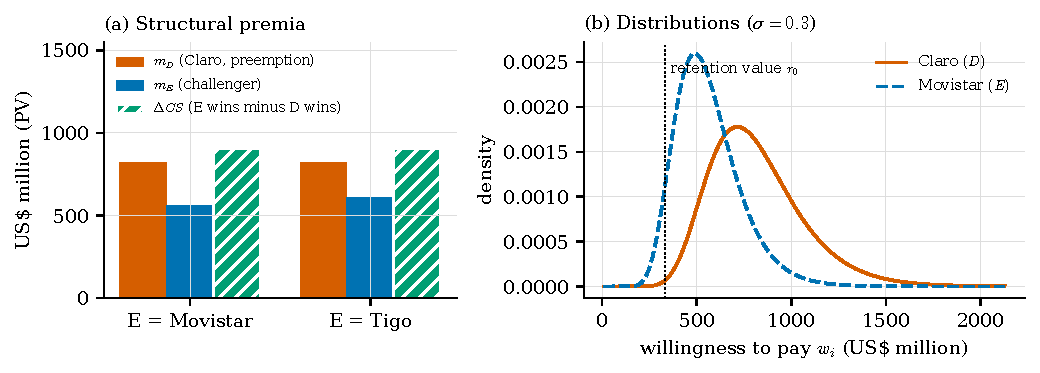
\includegraphics[width=0.95\textwidth]{figures/fig_premia_densities.pdf}
\caption{Structural premia and distributions of willingness to pay (baseline).}\label{fig:prem}
\end{figure}

\subsection{Three counterfactuals}

Table~\ref{tab:scen} and Figure~\ref{fig:welfare} give the main results.

\begin{table}[!htbp]
\centering\footnotesize
\caption{Counterfactual regimes: baseline calibration (Movistar as challenger; US\$ million, present value; Monte Carlo s.e.\ in parentheses; $N=10{,}000$)}\label{tab:scen}
\begin{tabular}{lcrrrrrrr}
\toprule
Scenario & $\beta$ & Net proceeds & Pr($D$) & Pr($E$) & Pr(none) & CS gain & E[HHI] & $\Delta W$ vs.\ S1 \\
\midrule
S1 Standard auction & 1.00 & 202 (1) & 0.82 & 0.18 & 0.00 & 165 (3) & 3,277 & 0 (5) \\
S2 Bid preference (beta*) & 0.44 & 109 (2) & 0.17 & 0.83 & 0.00 & 753 (3) & 3,148 & 359 (4) \\
S3 Set-aside (D barred) & -- & 0 (0) & 0.00 & 0.95 & 0.05 & 858 (2) & 3,124 & 331 (4) \\
Myerson benchmark & -- & 129 (2) & 0.15 & 0.82 & 0.02 & 746 (3) & 3,149 & 374 (4) \\
\bottomrule
\end{tabular}

\par\vspace{2pt}\scriptsize\textit{Notes:} Net proceeds are fiscal proceeds minus the retention value $r_0$. CS gain is the expected consumer surplus relative to the incumbent winning. $\Delta W$ is the planner's welfare $F+\kappa CS$ relative to S1 with $\kappa=\kappaBase$. The Myerson benchmark sells only if the winner's virtual value exceeds $r_0$.
\end{table}

\paragraph{S1: standard auction} Claro wins \pDStd\% of the time; expected net proceeds are \us\netStd{} million; the expected consumer-surplus gain relative to the incumbent always winning is only \us\csStd{} million, which comes from the \pEStd\% of auctions in which Movistar wins; expected HHI is \hhiStd.

\paragraph{S2: optimal bid preference} The welfare-maximising handicap is $\beta^*=\betaStar$. The challenger wins \pEPref\% of the time, expected net proceeds fall to \us\netPref{} million, a drop of \us\netDropPref{} million (\netLossPrefPct\%), and expected consumer surplus rises by \us\csGainPrefVsStd{} million relative to S1; the HHI falls to \hhiPref. Welfare rises by \us\dWPref{} million, \shareMyerson\% of the \us\dWMy{} million gain of the Myerson benchmark, which is the most that any incentive-compatible mechanism in our class can achieve.

\paragraph{S3: set-aside} Barring Claro gives the highest consumer-surplus gain (\us\csSA{} million) and the lowest HHI (\hhiSA), but the State obtains no surplus over its retention value: Movistar buys at the reserve whenever it qualifies and in \pNoSA\% of the cases the asset is not sold. Welfare rises by \us\dWSA{} million, less than under S2. By eliminating competition for the asset the set-aside forgoes the proceeds that the preference extracts from the incumbent's preemption motive.

\begin{figure}[!htbp]
\centering
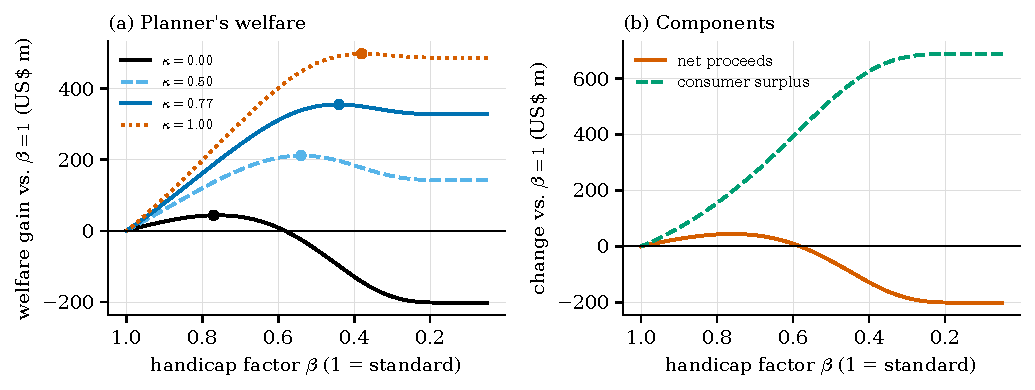
\includegraphics[width=0.95\textwidth]{figures/fig_welfare_beta.pdf}
\caption{Welfare as a function of the handicap $\beta$. Panel (a): welfare gain relative to $\beta=1$ for several weights $\kappa$ on consumer surplus (dots: maximisers). Panel (b): its components for the baseline $\kappa$.}\label{fig:welfare}
\end{figure}

\begin{figure}[!htbp]
\centering
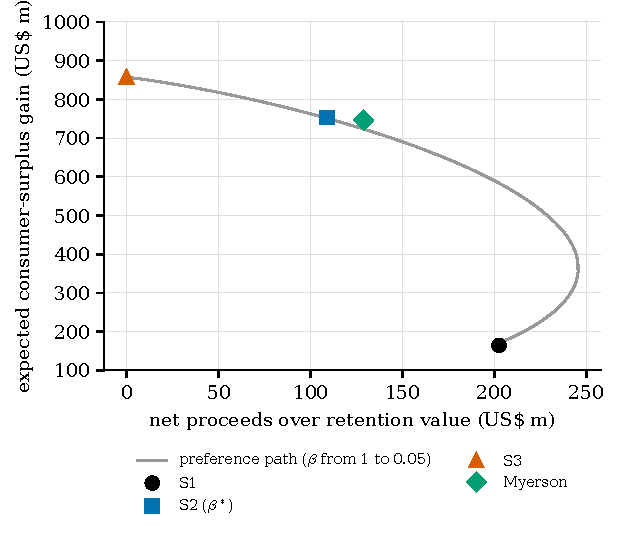
\includegraphics[width=0.6\textwidth]{figures/fig_frontier.pdf}
\caption{Revenue--consumer-surplus frontier. The grey path traces the handicap $\beta$ from 1 (S1) to 0.05, approaching the set-aside (S3).}\label{fig:frontier}
\end{figure}

\paragraph{A revenue-maximising State} With $\kappa=0$, Proposition~\ref{prop:handicap}(c) implies that a preference still raises proceeds. The optimal handicap is $\beta^*=\betaStarRev$ and net proceeds rise by \revGainPct\% (\us\revGainAbs{} million). A State indifferent to consumers would nonetheless favour the challenger, but the preference needed is much milder.

\begin{figure}[!htbp]
\centering
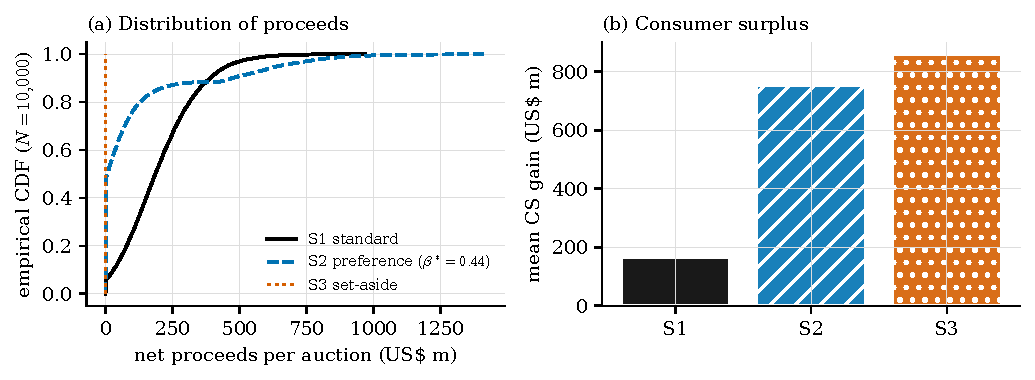
\includegraphics[width=0.95\textwidth]{figures/fig_ecdf.pdf}
\caption{Distribution of net proceeds across auctions and mean consumer-surplus gain (baseline, $N=10{,}000$).}\label{fig:ecdf}
\end{figure}

\clearpage
\subsection{Sensitivity}\label{sec:sensitivity}

Table~\ref{tab:sens} varies one parameter at a time and Figure~\ref{fig:heat} shows $\beta^*$ over $\sigma$ and $\kappa$. Across all runs $\beta^*$ lies between \betaMin{} and \betaMax{}; a preference for the challenger is always optimal ($\beta^*<1$). The handicap is stronger (lower $\beta^*$) when consumers carry more weight ($\beta^*=\betaKappaOne$ at $\lambda=0$ against $\lamZeroBeta$ for a pure revenue maximiser), when private valuations are more dispersed ($\betaSigmaLo$ at $\sigma=0.1$ against $\betaSigmaHi$ at $\sigma=0.6$, because a small handicap then changes few outcomes) and, mildly, when the asset is larger ($\betaDKLo$ to $\betaDKHi$ as $\Delta$ rises from 0.05 to 0.20). It is weaker when the market is measured by mobile Internet accesses or revenue ($\beta^*=\betaInternet$ and $\betaRevenue$), although the HHI is then higher. Because the set-aside is the limit $\beta\to0$ of the preference family, the optimal preference weakly dominates it by construction; the gap is small when $\kappa=1$ (about \us\gapSAKappaOne{} million) and large when the planner values revenue ($\kappa\le0.5$), where barring the incumbent can even be worse than the standard auction ($\kappa\le0.25$). Positive correlation between the private shocks (Section~\ref{sec:model}) strengthens, rather than weakens, the case for a preference: correlation reduces the dispersion of the ratio $w_D/w_E$, so the incumbent's structural advantage is less often overturned by private news. With a correlation of 0.75 the challenger wins only \pEStdCorrHi\% of standard auctions, the optimal handicap is milder ($\beta^*=\betaCorrHi$, because a given handicap then shifts more outcomes), and the welfare gain of the preference rises to \us\wGainCorrHi{} million, at expected net proceeds of \us\netPrefCorrHi{} million. The Myerson benchmark, which assumes independence, is not reported in these rows.

\begin{figure}[!htbp]
\centering
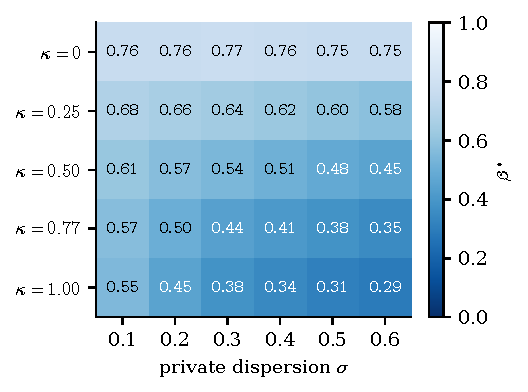
\includegraphics[width=0.55\textwidth]{figures/fig_heatmap_beta.pdf}
\caption{Optimal handicap $\beta^*$ as a function of the private dispersion $\sigma$ and the weight $\kappa$ on consumer surplus.}\label{fig:heat}
\end{figure}

\begin{table}[!htbp]
\centering\footnotesize
\caption{Sensitivity of the optimal handicap and welfare gains (US\$ million). Each row changes one baseline parameter}\label{tab:sens}
\resizebox{\textwidth}{!}{\begin{tabular}{lrrrrrrrrr}
\toprule
Value & $\beta^*$ & Pr($E$) S1 & Pr($E$) S2 & $\Delta W$ S2 & $\Delta W$ S3 & Net S1 & Net S2 & HHI S1 & HHI S2 \\
\midrule
\multicolumn{10}{l}{\textit{Private dispersion $\sigma$}} \\
0.1 & 0.57 & 0.00 & 0.90 & 567 & 485 & 210 & 151 & 3,313 & 3,133 \\
0.2 & 0.50 & 0.09 & 0.86 & 456 & 423 & 208 & 122 & 3,297 & 3,141 \\
0.3 & 0.44 & 0.18 & 0.83 & 359 & 331 & 202 & 109 & 3,277 & 3,148 \\
0.4 & 0.41 & 0.25 & 0.78 & 290 & 255 & 197 & 116 & 3,265 & 3,158 \\
0.5 & 0.38 & 0.29 & 0.73 & 243 & 202 & 191 & 121 & 3,257 & 3,167 \\
0.6 & 0.35 & 0.32 & 0.71 & 209 & 160 & 185 & 121 & 3,251 & 3,172 \\
\midrule
\multicolumn{10}{l}{\textit{Cost of public funds $\lambda$}} \\
$\lambda{=}0$ ($\kappa{=}1.00$) & 0.38 & 0.18 & 0.89 & 502 & 491 & 202 & 63 & 3,277 & 3,136 \\
$\lambda{=}0.3$ ($\kappa{=}0.77$) & 0.44 & 0.18 & 0.83 & 359 & 331 & 202 & 109 & 3,277 & 3,148 \\
$\lambda{=}1$ ($\kappa{=}0.50$) & 0.54 & 0.18 & 0.70 & 215 & 144 & 202 & 183 & 3,277 & 3,174 \\
$\lambda{=}3$ ($\kappa{=}0.25$) & 0.64 & 0.18 & 0.56 & 112 & -29 & 202 & 230 & 3,277 & 3,202 \\
$\lambda\to\infty$ ($\kappa{=}0$) & 0.77 & 0.18 & 0.39 & 45 & -202 & 202 & 248 & 3,277 & 3,236 \\
\midrule
\multicolumn{10}{l}{\textit{Asset size $\Delta K$}} \\
0.05 & 0.47 & 0.21 & 0.82 & 162 & 146 & 108 & 60 & 3,285 & 3,204 \\
0.1 & 0.44 & 0.18 & 0.83 & 359 & 331 & 202 & 109 & 3,277 & 3,148 \\
0.15 & 0.41 & 0.15 & 0.84 & 593 & 557 & 283 & 147 & 3,282 & 3,137 \\
0.2 & 0.40 & 0.14 & 0.84 & 668 & 631 & 303 & 155 & 3,285 & 3,142 \\
\midrule
\multicolumn{10}{l}{\textit{Margin $\mu$}} \\
0.2 & 0.44 & 0.18 & 0.83 & 205 & 189 & 116 & 62 & 3,277 & 3,148 \\
0.3 & 0.44 & 0.18 & 0.83 & 308 & 284 & 174 & 93 & 3,277 & 3,148 \\
0.35 & 0.44 & 0.18 & 0.83 & 359 & 331 & 202 & 109 & 3,277 & 3,148 \\
0.4 & 0.44 & 0.18 & 0.83 & 411 & 378 & 231 & 125 & 3,277 & 3,148 \\
0.5 & 0.44 & 0.18 & 0.83 & 513 & 473 & 289 & 156 & 3,277 & 3,148 \\
\midrule
\multicolumn{10}{l}{\textit{Reserve ratio $r_0/\bar p$}} \\
0.3 & 0.47 & 0.18 & 0.81 & 360 & 198 & 373 & 296 & 3,277 & 3,152 \\
0.5 & 0.46 & 0.18 & 0.82 & 362 & 297 & 267 & 183 & 3,277 & 3,149 \\
0.625 & 0.44 & 0.18 & 0.83 & 359 & 331 & 202 & 109 & 3,277 & 3,148 \\
0.8 & 0.44 & 0.18 & 0.73 & 306 & 296 & 122 & 47 & 3,278 & 3,168 \\
\midrule
\multicolumn{10}{l}{\textit{Horizon $T$ (years)}} \\
10 & 0.44 & 0.18 & 0.83 & 259 & 239 & 146 & 79 & 3,277 & 3,148 \\
15 & 0.44 & 0.18 & 0.83 & 321 & 296 & 181 & 97 & 3,277 & 3,148 \\
20 & 0.44 & 0.18 & 0.83 & 359 & 331 & 202 & 109 & 3,277 & 3,148 \\
\midrule
\multicolumn{10}{l}{\textit{Challenger}} \\
Movistar & 0.44 & 0.18 & 0.83 & 359 & 331 & 202 & 109 & 3,277 & 3,148 \\
Tigo & 0.48 & 0.24 & 0.83 & 313 & 282 & 216 & 114 & 3,242 & 3,062 \\
\midrule
\multicolumn{10}{l}{\textit{Correlation $r_\xi$ of the private shocks}} \\
0 & 0.44 & 0.18 & 0.83 & 359 & 331 & 202 & 109 & 3,277 & 3,148 \\
0.25 & 0.47 & 0.15 & 0.82 & 386 & 347 & 207 & 122 & 3,285 & 3,149 \\
0.5 & 0.50 & 0.10 & 0.82 & 421 & 370 & 212 & 132 & 3,294 & 3,150 \\
0.75 & 0.54 & 0.03 & 0.82 & 480 & 404 & 216 & 150 & 3,307 & 3,150 \\
\midrule
\multicolumn{10}{l}{\textit{Market definition}} \\
mobile lines & 0.44 & 0.18 & 0.83 & 359 & 331 & 202 & 109 & 3,277 & 3,148 \\
mobile Internet accesses & 0.51 & 0.23 & 0.79 & 271 & 229 & 214 & 143 & 3,784 & 3,600 \\
mobile revenue & 0.57 & 0.27 & 0.76 & 198 & 145 & 216 & 158 & 4,327 & 4,091 \\
\bottomrule
\end{tabular}
}
\par\vspace{2pt}\scriptsize\textit{Notes:} $\Delta W$ S2, S3 = welfare gain relative to S1 (same $\kappa$). Net = net proceeds. $\beta^*$ is chosen on $200{,}000$ draws and all outcomes are evaluated on the same $N=10{,}000$ draws as in Table~\ref{tab:scen}, so that the baseline row (Movistar, $\sigma=0.3$, $\lambda=0.3$, lines) reproduces Table~\ref{tab:scen} exactly.
\end{table}

\subsection{Reserve price}

Table~\ref{tab:reserve} re-optimises the reserve for each regime. The standard auction benefits most from a higher reserve (optimal at about 1.75 times the retention value) but remains far below the preference auction, whose optimal reserve is the retention value: once the challenger is favoured, competition between bidders, not the reserve, supports proceeds.

\begin{table}[!htbp]
\centering\small
\caption{Optimal reserve by regime (baseline; US\$ million)}\label{tab:reserve}
\begin{tabular}{lcccccrr}
\toprule
Scenario & $\rho/r_0$ & $\beta$ & Net proceeds & Pr($E$) & Pr(none) & CS gain & $W-W_0$ \\
\midrule
S1 Standard & 1.75 & 1.00 & 261 & 0.16 & 0.10 & 141 & 370 \\
S2 Preference & 1.00 & 0.44 & 104 & 0.84 & 0.00 & 758 & 686 \\
S3 Set-aside & 1.05 & -- & 15 & 0.92 & 0.08 & 838 & 660 \\
\bottomrule
\end{tabular}

\par\vspace{2pt}\footnotesize\textit{Notes:} $\rho/r_0$: optimal reserve as a multiple of the retention value (grid 1--2). $W-W_0$: welfare relative to retaining the asset.
\end{table}

%% ---------------------------------------------------------------------------
\section{Discussion, extensions and limitations}\label{sec:discussion}

\subsection{Policy implications}

If a further privatisation of a mobile or converged operator occurs, our results suggest that the State should not run a standard auction against Claro. Counting the incumbent's bid at $\betaStar$ of its face value redirects the asset to a challenger most of the time at the cost of lower proceeds. This cost is the price of competition and should be reported as such. If the State is unwilling to sacrifice proceeds, a much milder handicap ($\beta=\betaStarRev$) is revenue-maximising. Barring the incumbent was never better than the optimal preference in our experiments, and is clearly worse when public revenue is valued. These conclusions are consistent with the Colombian legal framework, which makes free competition a guiding principle of ICT policy \citep{ley1341,ley1978}.

\subsection{Extension: more than one challenger}\label{sec:multi}

In practice both Movistar and Tigo could bid against Claro. With two constrained challengers $E_1,E_2$ the externality a challenger suffers depends on \emph{who} wins if it loses \citep{jehielmoldovanu2000}: if $D$ wins the margin stays at $P^0$, whereas if the other challenger wins the margin falls to $P^{E_2}<P^0$, and a constrained challenger, which sells its fixed capacity at the margin, loses profit. Table~\ref{tab:three} reports the pairwise premia implied by the calibrated model when Claro, Movistar and Tigo all bid. Movistar would pay \us\pairMvsC{} million to win rather than let Claro win, but \us\pairMvsT{} million to win rather than let Tigo win; the corresponding figures for Tigo are \us\pairTvsC{} and \us\pairTvsM{} million. Claro's premium is \us\pairCvsE{} million against either challenger.

\begin{table}[!htbp]
\centering\small
\caption{Pairwise premia with three bidders (US\$ million, present value): bidder $i$'s gain from winning rather than losing to the winner in each column}\label{tab:three}
\begin{tabular}{lrrr}
\toprule
Bidder $i$ & if Claro wins & if Movistar wins & if Tigo wins \\
\midrule
Claro & -- & 818 & 818 \\
Movistar & 561 & -- & 774 \\
Tigo & 611 & 774 & -- \\
\bottomrule
\end{tabular}

\par\vspace{2pt}\footnotesize\textit{Notes:} Calibrated downstream model; both challengers' capacity expansion equals $\Delta$; $\pi_i^i-\pi_i^j$.
\end{table}

Three implications follow. First, a challenger's willingness to pay is no longer a single number. In an ascending auction with three bidders, drop-out prices depend on which rivals remain, so the dominant-strategy reduction of Lemma~\ref{lem:wtp} does not extend and the equilibrium must be solved numerically. Second, the challengers have no common interest in blocking the dominant firm: each prefers a victory by $D$ to a victory by its rival, since $\pi_{E_1}^{D}>\pi_{E_1}^{E_2}$. The collective-action problem is therefore not free-riding on a shared benefit, because a constrained challenger is hurt when the other expands; it is mutual denial, and neither internalises the consumer-surplus and concentration gains that the planner obtains whenever \emph{any} challenger wins. Third, the net effect on the incumbent's probability of winning a standard auction is ambiguous, because mutual denial raises the challengers' bids against each other but does not coordinate them against $D$. A handicap applied to $D$'s bid, by contrast, does not require coordination among challengers, which strengthens the case for the instrument; we leave the numerical solution of the three-bidder game to future research.

\subsection{Extension: an informational advantage}\label{sec:insider}

The main model treats market dominance. Informational asymmetries are a distinct problem, and we treat one as a self-contained benchmark. Suppose the object has a common value $V=X+Y$, where $X$ is public (e.g.\ the State's independent valuation) and $Y\sim U[0,s]$ is observed only by an \emph{insider}; the \emph{outsider} knows only the distribution of $Y$ \citep{emw1983}.

\begin{proposition}[Informational advantage]\label{prop:insider}
In the sealed first-price auction the insider bids $X+y/2$ and the outsider randomises over the same distribution, earning zero. Expected revenue is $R_{FP}=X+s/3$ and the insider's rent is $s/6$. If $Y$ is disclosed to both bidders, price equals $V$ and $R_{FI}=X+s/2$. The loss from the informational advantage is $s/6$, one third of the expected surplus above $X$.
\end{proposition}

Disclosure of the information in the sale process (data rooms, public financial statements) is the remedy; bid preferences are not, since they do not change who knows what \citep{milgromweber1982}. As an illustration for 2006, taking the State's valuation as $X$ and treating the realised price as $R_{FP}$ gives an implied dispersion $s=3(R-X)=\us\coltelS{}$ million and an illustrative magnitude for the insider's rent of \us\coltelLossUSD{} million (\coltelLossPct\% of the price; Table~\ref{tab:informed}). The public record does not establish that any bidder in 2006 held such an advantage, and the exercise applies to a sealed first-price rule whereas the 2006 sale was ascending, a format that can transmit information and therefore need not reproduce this result.

\begin{table}[!htbp]
\centering\small
\caption{Illustrative cost of an informational advantage, COLTEL 2006}\label{tab:informed}
\begin{tabular}{lrr}
\toprule
Item & COP million & USD million \\
\midrule
Reserve (State valuation, $X$) & 533,577 & 231 \\
Realised price ($R_{FP}$) & 853,577 & 369 \\
Implied dispersion $s=3(R-X)$ & 960,000 & 415 \\
Insider rent $s/6$ & 160,000 & 69 \\
Counterfactual price under disclosure $X+s/2$ & 1,013,577 & 438 \\
\bottomrule
\end{tabular}

\par\vspace{2pt}\footnotesize\textit{Notes:} $X$ = minimum price set from Citigroup/McKinsey valuations; $R_{FP}$ = winning bid; implied by Proposition~\ref{prop:insider} with uniform $Y$. USD at 2,313 COP per USD (implied by \citealt{infobae2006}). Illustrative only, see text.
\end{table}

\subsection{Limitations}\label{sec:limitations}

First, the downstream model is stylised: capacity-constrained Cournot with linear demand, a single dominant firm and two bidders. Price-setting formulations with capacity limits may give different margins (Section~\ref{sec:model}). The size of the consumer-surplus gains rests on that structure and the capacity parameter $\Delta$, so absolute magnitudes should be read as illustrative, and we recommend the sensitivity analysis over the baseline. Second, the dispersion of private values is not identified from market data, and we assume independent shocks across bidders (relaxed numerically in Section~\ref{sec:sensitivity}); estimating both requires bid data. Third, we abstract from strategic non-participation and from the seller's ability to exploit externalities further (Assumption~\ref{ass:sale}); both may change the seller's optimal mechanism \citep{jms1996}, so our benchmarks should be read within the class defined by that assumption. Fourth, we model two bidders and leave the three-bidder auction to future work (Section~\ref{sec:multi}). Fifth, we do not model collusion or post-auction regulation (access, caps, mandated roaming), which are substitutes for the discrimination studied here. Finally, we do not analyse first-price formats; Lemma~\ref{lem:wtp} implies that the standard asymmetric-auction theory applies to willingness to pay \citep{maskinriley2000,cantillon2008}, so this extension is tractable numerically.

%% ---------------------------------------------------------------------------
\section{Conclusion}\label{sec:conclusion}

In concentrated telecommunications markets the dominant firm values a privatised asset in part because it denies the asset to its rivals. We show in a calibrated model that a standard ascending auction then hands the asset to the incumbent with a probability of \pDStd\% even though consumers would be better off if a challenger won. A bid preference for the challenger is dominant-strategy incentive compatible, captures most of the gain of the optimal mechanism, and dominates barring the incumbent. The cost, lower expected proceeds, is explicit, and the preference remains attractive even for a pure revenue maximiser. Informational advantages call for a different instrument, disclosure. Extensions include estimating bidder heterogeneity from bids, solving the three-bidder game, a richer downstream market with differentiated products, multi-unit spectrum auctions, and dynamic post-sale regulation.

\section*{Declarations}
\noindent\textbf{Funding:} The author received no specific funding for this work.\\
\textbf{Competing interests:} The author has no competing interests to declare.\\
\textbf{Author contributions:} Single-authored.\\
\textbf{Data and code availability:} All data are public (MinTIC and the sources cited above). The data and the code that generates every number, table and figure of this paper are available at \repourl{} (version archived with a DOI on Zenodo upon acceptance); see Appendix~\ref{app:repro}.

\appendix
\section{Proofs}\label{app:proofs}

\begin{proof}[Proof of Lemma~\ref{lem:cournot}]
Firm $j$'s profit $q_j(\bar a-Q_{-j}-q_j)$ is strictly concave, so the best response is $\min\{k_j,\max\{0,(\bar a-Q_{-j})/2\}\}$. In an equilibrium with margin $P=\bar a-Q$ the unconstrained optimum of firm $j$ is $(\bar a-Q_{-j})/2=(P+q_j)/2$. Firm $j$ is therefore at capacity if and only if $(P+k_j)/2\ge k_j$, i.e.\ $k_j\le P$, and otherwise chooses $q_j=P$ (as $(P+q_j)/2=q_j$). Hence $q_j=\min\{k_j,P\}$ and $P$ solves $g(P)\equiv P+\sum_j\min\{k_j,P\}=\bar a$. $g$ is continuous, strictly increasing, $g(0)=0<\bar a$ and $g\to\infty$, so $P$ exists and is unique. Totally differentiating, $dP/dk_j=-\mathbf 1\{k_j<P\}/g'(P)<0$ if $k_j<P$ and $0$ otherwise, with $g'(P)=1+\#\{i:k_i>P\}\ge1$.
\end{proof}

\begin{proof}[Proof of Proposition~\ref{prop:preemption}]
(a) By Assumption~\ref{ass:dominance} and Lemma~\ref{lem:cournot}, $D$ is unconstrained ($k_D\ge P^0$), so its extra capacity does not change the equilibrium and $P^D=P^0$. If $E$ wins, $k_E+\Delta>k_E$ with $k_E<P^0$, so $P^E<P^0$; $Q=a-P$ and $CS=(a-P)^2/2$ give the claim. (b) $D$ is unconstrained, so $q_D=P$ and $\pi_D=P^2$; $D$'s gain from the asset is zero because capacity is slack, and $m_D=\Gamma\Lambda[(P^D)^2-(P^E)^2]>0$ by (a). (c) With $a=1$ and $k_E=x<1/3$: if $D$ wins, $q_D=(1-x)/2$, $P=(1-x)/2$, $\pi_D=(1-x)^2/4$, $\pi_E=x(1-x)/2$; if $E$ wins and $\Delta\ge1/3-x$ both produce $1/3$, $P=1/3$, $\pi_i=1/9$. This gives $m_D$ and $m_E$, and $(1-x^2)/4-2/9>0\iff x<1/3$. $D$'s share is $q_D/(q_D+k_E)=(1-x)/(1+x)>1/2$. Total surplus is $CS+\Pi=(1+x)(3-x)/8$ when $D$ wins and $4/9$ when $E$ wins; the difference $g(x)=4/9-(3+2x-x^2)/8$ satisfies $g(1/3)=0$, $g'(x)=-(1-x)/4<0$, hence $g>0$ on $[0,1/3)$. The HHI is $((1-x)^2+4x^2)/(1+x)^2\ge1/2$ when $D$ wins and $1/2$ when $E$ wins.
\end{proof}

\begin{proof}[Proof of Lemma~\ref{lem:wtp}]
Fix the rival's bid. A bidder wins iff its bid exceeds a threshold $\tau$ that depends only on the rival's bid, $\beta$ and $\rho$, and pays $\tau$ on winning. By Assumption~\ref{ass:sale}(ii) its payoff when losing is the payoff of non-participation, so the difference between winning and losing is $w_i-\tau$. It prefers to win if and only if $w_i\ge\tau$, which truthful bidding $b_i=w_i$ achieves for every $\tau$. Qualification requires $w_i\ge\rho$ by Assumption~\ref{ass:sale}(i).
\end{proof}

\begin{proof}[Proof of Proposition~\ref{prop:myerson}]
Let $x_i(w)$ and $p_i(w)$ be the allocation and payment, $X_i,T_i$ their interim expectations and $U_i(w_i)=w_iX_i(w_i)-T_i(w_i)$ the net gain over losing. Bayesian incentive compatibility is equivalent to $X_i$ non-decreasing and $U_i(w_i)=U_i(\underline w_i)+\int_{\underline w_i}^{w_i}X_i$; individual rationality is $U_i(\underline w_i)\ge0$. Integrating by parts, $\E[T_i]=\E[x_i\psi_i(w_i)]-U_i(\underline w_i)$. The planner's welfare \eqref{eq:W} is $\E[\sum_i(p_i+\kappa x_i\Gamma\Lambda(CS^i-CS^D))+(1-\sum_ix_i)r_0]+\kappa\Gamma\Lambda CS^D$, since $CS^\varnothing=CS^D$, so
\[
W=\kappa\Gamma\Lambda CS^D+r_0+\E\Big[\sum_ix_i\big(\psi_i(w_i)+\theta_i-r_0\big)\Big]-\sum_iU_i(\underline w_i).
\]
Pointwise maximisation sets $U_i(\underline w_i)=0$ and $x_i=1$ for the bidder with the highest $\psi_i+\theta_i$ if it exceeds $r_0$. Under regularity this rule is monotone in $w_i$, so the incentive-compatibility conditions hold, and with critical-value payments it is dominant-strategy implementable. Statement (i) follows because $\psi_E\ge\psi_D$ ranks $E$ first on ties; (ii) is immediate from the allocation rule.
\end{proof}

\begin{proof}[Proof of Proposition~\ref{prop:handicap}]
(a) is the critical-bid rule: given $b_E$, $D$ wins iff $b_D>b_E/\beta$ and pays $b_E/\beta$; given $b_D$, $E$ wins iff $b_E>\beta b_D$ and pays $\beta b_D$; payments are at least $\rho$, and the proof of Lemma~\ref{lem:wtp} gives dominance and ex-post individual rationality. (b) The lowest qualified type $w=\rho$ never obtains positive surplus, so $U_i(\rho)=0$ and the revenue identity in the proof of Proposition~\ref{prop:myerson} applies with allocation restricted to qualified bidders. As $\beta\downarrow0$, $\beta w_D<w_E$ for all finite $w_D$, so $E$ wins whenever qualified and pays $\max\{\rho,\beta w_D\}\to\rho$; if only $D$ qualifies it wins and pays $\rho$, which is why the limit coincides with the set-aside only on $\{w_E\ge\rho\}$. (c) By the identity of (b), $W=\mathrm{const}+\E\big[\sum_ix_i^\beta(\psi_i+\theta_i)\mathbf 1\{w_i\ge\rho\}\big]+r_0\Pr(\text{none})$. Lowering $\beta$ from $1$ to $1-\epsilon$ changes the allocation only on $\{w_E<w_D\le w_E/\beta,\,w_E\ge\rho\}$, from $D$ to $E$, a set of probability $\epsilon\int w f_D(w)f_E(w)dw+o(\epsilon)$ on which $w_D=w_E=w$ to first order. The welfare change per reallocation is $\psi_E(w)+\theta-\psi_D(w)$, giving the derivative. The sign conditions follow.
\end{proof}

\begin{proof}[Proof of Proposition~\ref{prop:uniform}]
Take $k=1$ (everything scales with $k$). (b) For $\beta\in[\alpha,1]$ and $w_E\le\alpha\le\beta$, $D$ wins when $w_D\ge w_E/\beta$ (within the support) and pays $w_E/\beta$:
$\frac1\alpha\int_0^\alpha\!\frac{w}{\beta}\big(1-\frac w\beta\big)dw=\frac{\alpha}{2\beta}-\frac{\alpha^2}{3\beta^2}$. $E$ wins when $w_D<w_E/\beta$ and pays $\beta w_D$: $\frac1\alpha\int_0^\alpha\!\int_0^{w/\beta}\beta v\,dv\,dw=\frac{\alpha^2}{6\beta}$. Summing gives $R(\beta)=\frac{\alpha}{6\beta}(3+\alpha-2\alpha/\beta)$; $R(1)=\alpha/2-\alpha^2/6$ is (a). Setting $R'(\beta)=0$ gives $\beta^*=4\alpha/(3+\alpha)\in[\alpha,1]$ and $R(\beta^*)=(3+\alpha)^2/48$; hence the gain is $\frac{(3+\alpha)^2}{48}-\frac{3\alpha-\alpha^2}{6}=\frac{3(1-\alpha)^2}{16}$. (c) Here $\psi_D(w)=2w-1$ and $\psi_E(w)=2w-\alpha$, so $D$ wins iff $2w_D-1\ge2w_E-\alpha+t$, i.e.\ $w_D\ge w_E+\delta$ with $\delta=\tfrac12(1-\alpha+t)$. The frontier meets the top edge of $E$'s support, $w_E=\alpha$, at $w_D=\alpha+\delta=\frac{1+\alpha+t}{2}$, which is at most $1$ if and only if $t\le1-\alpha$; and it meets the right edge $w_D=1$ at $w_E=1-\delta$, which lies in $[0,\alpha]$ if and only if $1-\alpha\le t\le1+\alpha$. For $t\le1-\alpha$,
\[
V=\frac1\alpha\int_0^\alpha\Big[\int_{w+\delta}^{1}(2v-1)\,dv+\int_0^{w+\delta}(2w-\alpha+t)\,dv\Big]dw=\frac{3+\alpha^2+6t+3t^2}{12}.
\]
For $1-\alpha<t\le1+\alpha$ the first integral runs over $w\in[0,1-\delta]$ only, and for $w\in(1-\delta,\alpha]$ bidder $E$ wins for every $w_D$:
\begin{equation}\label{eq:Vii}
V=\frac1\alpha\Big[\int_0^{1-\delta}\!\!\Big(\int_{w+\delta}^{1}(2v-1)\,dv+\int_0^{w+\delta}(2w-\alpha+t)\,dv\Big)dw+\int_{1-\delta}^{\alpha}(2w-\alpha+t)\,dw\Big]
=\frac{\alpha^3-3\alpha^2t+3\alpha^2+3\alpha t^2+18\alpha t+3\alpha-t^3+3t^2-3t+1}{24\alpha}.
\end{equation}
For $t>1+\alpha$ we have $\delta>1$, $D$ never wins and $V=\E[2w_E-\alpha+t]=t$. Restoring the scale, $V(\theta)=k\,V(t)$. At $\theta=0$ the first case gives $(3+\alpha^2)k/12$. Each regime was verified symbolically and by Monte Carlo (\texttt{tests/test\_auctions.py}). (d) $\frac{3(1-\alpha)^2/16}{(1-\alpha)^2/4}=\frac34$. Symbolic and numerical confirmations are in \texttt{scripts/audit\_original.py} and \texttt{tests/}.
\end{proof}

\begin{proof}[Proof of Proposition~\ref{prop:insider}]
Let the insider bid $X+y/2$. An outsider bidding $X+t/2$ wins iff $Y<t$ and earns $\frac1s\int_0^t\big(y-t/2\big)dy=0$ for every $t$, so any bid distribution is a best response; mimicking the insider's bid distribution makes the insider indifferent to the distribution of its own bid only if $b(y)=X+y/2$: the insider with type $y$ maximises $(y-u)\,2u/s$ over $u=b-X$, whose optimum is $u=y/2$. Revenue is $X+\E\max\{Y_1,Y_2\}/2=X+s/3$ and the insider's expected profit is $\E[y^2/2]/s=s/6$. Under disclosure both know $V$, Bertrand competition gives price $V$ and expected revenue $X+s/2$.
\end{proof}

\section{Data and calibration details}\label{app:data}

Raw MinTIC figures (lines, mobile Internet accesses, revenue by operator, fixed Internet accesses) and COLTEL facts, with page and figure references, are in \texttt{data/raw/}. The HHI and the dominance threshold in Table~\ref{tab:market} are computed directly from the MinTIC shares, treating unlisted operators as an atomistic fringe (which yields a lower bound for the HHI). COP/USD is the 2020 average market rate of 3,693 (approximate); the 2006 conversion of 2,313 is implied by \citet{infobae2006}. Table~\ref{tab:scen-tigo} repeats the main experiment with Tigo as the challenger.

\begin{table}[!htbp]
\centering\footnotesize
\caption{Counterfactual regimes with Tigo as the challenger (US\$ million)}\label{tab:scen-tigo}
\begin{tabular}{lcrrrrrrr}
\toprule
Scenario & $\beta$ & Net proceeds & Pr($D$) & Pr($E$) & Pr(none) & CS gain & E[HHI] & $\Delta W$ vs.\ S1 \\
\midrule
S1 Standard auction & 1.00 & 216 (1) & 0.76 & 0.24 & 0.00 & 217 (4) & 3,242 & 0 (5) \\
S2 Bid preference (beta*) & 0.48 & 114 (2) & 0.17 & 0.83 & 0.00 & 756 (3) & 3,062 & 313 (4) \\
S3 Set-aside (D barred) & -- & 0 (0) & 0.00 & 0.95 & 0.05 & 865 (2) & 3,026 & 282 (4) \\
Myerson benchmark & -- & 132 (2) & 0.15 & 0.83 & 0.03 & 749 (3) & 3,064 & 326 (4) \\
\bottomrule
\end{tabular}

\end{table}

\section{Reproducibility}\label{app:repro}

The replication package is a Python project (\texttt{src/privauction}) with data, tests and a single entry point. The command \texttt{python scripts/run\_all.py} regenerates every table and figure and the file \texttt{numbers.tex} that supplies all numerical values quoted in the text, so that text and results cannot diverge. Tests check the downstream equilibrium against an independent best-response iteration, the closed forms of Propositions~\ref{prop:preemption}, \ref{prop:uniform} and~\ref{prop:insider} against Monte Carlo, dominant-strategy incentive compatibility by brute force, the payment identity of Proposition~\ref{prop:myerson}, and that the Myerson mechanism weakly dominates all other regimes. All random draws use fixed seeds.

\bibliographystyle{apalike}
\bibliography{references}

\end{document}
